% CVPR 2026 Submission
\documentclass[10pt,twocolumn,letterpaper]{article}

% CVPR/ICCV style — [review] for submission, [final] for a clean local PDF
\usepackage[final]{iccv}

\def\confName{CVPR}
\def\confYear{2026}
\def\paperID{****}

\usepackage[utf8]{inputenc}
\usepackage[T1]{fontenc}
\usepackage[breaklinks,colorlinks]{hyperref}
\usepackage{nicefrac}
\usepackage{microtype}
\usepackage{graphicx}
\usepackage{multirow}
\usepackage{tabularx}
\usepackage{xcolor}

\newcounter{algorithm}
\newenvironment{cvpralgorithm}{\begin{figure}[t]\refstepcounter{algorithm}\noindent\begin{minipage}{\linewidth}}{\end{minipage}\end{figure}}
\newcommand{\algorithmcaption}[1]{\noindent\emph{Algorithm \thealgorithm. #1}\par\vspace{2pt}}
\newcommand{\algkw}[1]{\emph{#1}}
\newcommand{\algindent}{\hspace*{1.2em}}
\newcommand{\algindenttwo}{\hspace*{2.4em}}

\title{Monocular Geometry Is Enough: \\ Depth-Conditioned Pseudo-Labels for \\ Scene-Centric Unsupervised Panoptic Segmentation}

\author{Anonymous CVPR 2026 Submission \\
Paper ID \paperID}

\begin{document}
\raggedbottom

\maketitle

\begin{abstract}
Panoptic segmentation assigns a category to every pixel and a distinct identity to every countable object, and underpins autonomous driving, robotic perception, and dense scene understanding. Scene-centric unsupervised methods replace human masks with pseudo-labels, but CUPS constructs those labels using stereo depth and motion cues at pseudo-label time. This restricts the setting to footage captured with multi-view or temporal input, while most available imagery is monocular.

We study whether monocular cues can provide the same pseudo-label structure. Frozen semantic codes provide category-consistent regions, monocular depth provides physical separation cues, and dense self-supervised features test whether adjacent fragments have compatible appearance. We combine these cues with two mechanisms: a depth-conditioned residual adapter (DCFA) for the semantic code and Semantic Instance Mutual Consistency Filtering (SIMCF) for candidate labels. On Cityscapes, DCFA improves semantic mIoU from 52.69 to 55.29, and DCFA+SIMCF improve pseudo-label PQ from 24.54 to 25.85 before panoptic bootstrapping. After CUPS-style panoptic bootstrapping and panoptic network training, the final model yields 35.83 PQ, 62.79 SQ, and 43.78 RQ on Cityscapes val, compared with 32.76 PQ for the corresponding monocular baseline without DCFA/SIMCF and 27.80 PQ for the published CUPS configuration.
\end{abstract}

\begin{figure*}[t]
\centering
\includegraphics[width=\textwidth]{../figures/paper_ready/pipeline_overview.png}
\caption{Pipeline overview. Stage 1 constructs panoptic pseudo-labels from a single RGB image using frozen semantic features, monocular depth, DCFA, and SIMCF. Stage 2 adopts CUPS-style panoptic bootstrapping and panoptic network training on the filtered labels.}
\label{fig:pipeline_overview}
\end{figure*}


%=========================================================================
\section{Introduction}
\label{sec:intro}
%=========================================================================

Panoptic segmentation assigns a category to every pixel and a distinct identity to every countable object. The task underpins autonomous driving, robotic manipulation, and dense scene parsing, and its supervised counterpart sits at the top of every benchmark that supplies dense human masks. The obstacle is annotation cost: Cityscapes-style annotation requires a pixel-level mask for every visible instance, and the cost compounds with each new dataset and domain. The unsupervised setting asks whether a model can recover panoptic structure from raw pixels alone.

Recent progress has come from three lineages. Self-supervised semantic discovery on top of frozen DINO/DINOv2 features~\cite{caron2021dino,oquab2024dinov2} now yields region-level partitions coherent enough to serve as semantic pseudo-labels~\cite{hamilton2022stego,kim2024cause}. Cut-and-learn instance discovery~\cite{simeoni2021lost,wang2023tokencut,wang2023cutler} extracts foreground masks from the same SSL features and bootstraps detectors from them. CutS3D~\cite{sick2025cuts3d} moves this instance line toward scene-centric data by lifting depth to a 3-D point cloud and applying LocalCut to disambiguate adjacent instances. CUPS~\cite{hahn2025cups} combines semantic pseudo-labels, stereo-derived depth, and unsupervised scene flow, then trains a Cascade Mask R-CNN with DropLoss bootstrapping and EMA self-training.

CUPS obtains this structure from calibrated stereo at pseudo-label time and unsupervised optical flow over short video clips. These inputs are not available for many scene-centric datasets, where images often arrive as single monocular frames from a phone, dashcam, or fixed camera. A method that depends on multi-view input therefore narrows the range of imagery where unsupervised panoptic segmentation can be applied. We ask whether this extra input is necessary, or whether monocular images already contain enough structure for pseudo-label generation.

We show that frozen monocular priors can replace stereo and motion at pseudo-label time when they are combined through cross-modal agreement. Semantic codes provide class-consistent regions but may merge adjacent same-class objects or split a surface under illumination change. Monocular depth provides physical separations but may over-fragment objects along material seams. Dense feature similarity can merge depth fragments when their appearance is compatible. Our pipeline uses these cues conservatively: depth proposes candidate boundaries, while semantic identity and feature similarity decide which boundaries should survive.

This design improves pseudo-label panoptic quality from 24.54 to 25.85 on Cityscapes before panoptic bootstrapping. After CUPS-style panoptic bootstrapping and panoptic network training, the final model reaches 35.83 PQ, 62.79 SQ, and 43.78 RQ on Cityscapes val. The corresponding monocular baseline without DCFA/SIMCF reaches 32.76 PQ under the same training procedure, isolating a +3.07 PQ gain from the proposed pseudo-label generator. The published CUPS configuration reaches 27.80 PQ with stereo + motion cues at pseudo-label time.

We make three contributions:
\begin{itemize}
\item Stereo-and-motion-free pseudo-label generation for scene-centric panoptic segmentation. Monocular semantic appearance and monocular depth, composed by an agreement filter, supply enough structure for scene-centric unsupervised panoptic-label generation, removing CUPS's stereo + motion requirement at pseudo-label time.
\item Two compact mechanisms for cross-modal agreement. A depth-conditioned residual adapter (DCFA) adapts a frozen 90-dimensional semantic code toward depth-consistent regions and lifts semantic mIoU from 52.69 to 55.29; Semantic Instance Mutual Consistency Filtering (SIMCF) accepts, revises, or rejects candidate labels through semantic, geometric, and appearance agreement and contributes the bulk of the +1.31 PQ pseudo-label gain.
\item 35.83 PQ on Cityscapes after panoptic network training. Using the adopted CUPS panoptic bootstrapping and network-training procedures, the final network reaches 35.83 PQ on Cityscapes val, a +3.07 PQ gain over the corresponding monocular baseline.
\end{itemize}

Figure~\ref{fig:pipeline_overview} gives the full pipeline view. Section~\ref{sec:related} surveys the unsupervised semantic, instance, and panoptic literatures. Section~\ref{sec:method} develops the pipeline. Section~\ref{sec:experiments} reports Cityscapes results, ablations, and transfer experiments. Section~\ref{sec:discussion} discusses the results. Section~\ref{sec:limitations} summarizes the main limitations.

%=========================================================================
\section{Related Work}
\label{sec:related}
%=========================================================================

\paragraph{Unsupervised Semantic Segmentation.}
Early unsupervised semantic segmentation methods optimized clustering objectives over learned image representations: IIC~\cite{ji2019iic} maximized mutual information between augmented views, and PiCIE~\cite{cho2021picie} enforced photometric and geometric invariance to recover pixel-level groupings. The arrival of self-supervised vision transformers~\cite{caron2021dino,oquab2024dinov2} reshaped the field, with dense ViT features clustering cleanly enough that \emph{distillation} methods became dominant. STEGO~\cite{hamilton2022stego} distilled DINO correspondences into compact dense embeddings; HP~\cite{seong2023hp} improved this contrastive pool by discovering hidden positives; CAUSE~\cite{kim2024cause} structured the latent space through a concept clusterbook, producing a concept-coherent semantic code. Recent variants refine the clustering objective on top of these SSL features but do not change what is being clustered: spectral aggregation in EAGLE~\cite{kim2024eagle}, proxy-anchor mining in PPAP~\cite{seong2024ppap}, diffusion-feature partitioning in DiffCut~\cite{couairon2024diffcut}, and recursive hierarchy clustering~\cite{bonnet2024hierarchy}.

Monocular depth has been considered as an auxiliary signal throughout this lineage. DepthG~\cite{sick2024depthg} adds a depth-feature correlation loss together with depth-guided positive/negative sampling on top of a STEGO-style backbone, while CUPS~\cite{hahn2025cups} uses depth as a contrastive auxiliary in its DINO-distillation semantic head. Earlier work used depth as a multi-task pre-training signal~\cite{hoyer2021threeways}. In a separate, fully \emph{supervised} line, RGB-D fusion methods inject depth into attention but require dense labels (DFormerv2~\cite{yin2025dformerv2}). Unlike these prior unsupervised depth-guided methods that use depth as a loss-side signal or sampling prior, DCFA conditions a frozen unsupervised semantic code on monocular depth through a small residual adapter, leaving the backbone untouched.

\paragraph{Unsupervised Instance Segmentation.}
The dominant line of unsupervised instance discovery applies graph-cut-style partitioning to self-supervised features. LOST~\cite{simeoni2021lost} localized a single salient object per image; TokenCut~\cite{wang2023tokencut} generalized this through normalized cuts on DINO patch tokens; MaskCut~\cite{wang2023cutler} iterated TokenCut to extract multiple masks per image; CutLER~\cite{wang2023cutler} turned MaskCut pseudo-masks into supervision for a class-agnostic Cascade Mask R-CNN, establishing the cut-and-learn template. MaskDistill~\cite{vangansbeke2022maskdistill} and FreeSOLO~\cite{wang2022freesolo} explored alternative pseudo-mask formulations within the same paradigm.

Recent extensions diversify the cut-and-learn template. CuVLER~\cite{arica2024cuvler} strengthens MaskCut with multi-SSL feature voting and soft-target distillation; COLER~\cite{feng2025coler} cuts in a single pass without k-means; ProMerge~\cite{li2024promerge} introduces prompt-and-merge grouping with background-based pruning; unMORE~\cite{yang2025unmore} learns existence/center/boundary fields; UnSAM and UnSAMv2~\cite{wang2024unsam,yu2025unsamv2} add granularity-controlled segmentation on SA-1B-scale data. Slot-attention models such as DINOSAUR~\cite{seitzer2023dinosaur} and its motion-refined extension MR-DINOSAUR~\cite{gong2025mrdinosaur} are adjacent alternatives that largely target object-centric or class-agnostic instance discovery rather than the instance branch of scene-centric panoptic pseudo-labeling.

A separate subline injects geometric information explicitly, and CutS3D~\cite{sick2025cuts3d} is the closest comparison to our instance pipeline. CutS3D lifts each image to a 3-D point cloud through monocular depth, constructs a 3-D k-NN graph, and applies LocalCut to disambiguate adjacent instances that 2-D NCut merges. We share CutS3D's monocular premise but stay entirely in 2-D: depth gradients provide a 2-D proxy for the separation cue CutS3D obtains after unprojecting depth to 3-D, namely local discontinuities between physically distinct surfaces. After Sobel filtering and connected-component analysis within thing-eligible semantic regions, this 2-D treatment supplies the instance side of our pseudo-labels without lifting to a point cloud or constructing a 3-D graph.

\paragraph{Unsupervised Panoptic Segmentation.}
Unsupervised panoptic segmentation is a young task. The most directly comparable Cityscapes results to date come from three works. U2Seg~\cite{niu2024u2seg} is the first unified framework, composing STEGO and MaskCut on object-centric data and transferring to scene-centric Cityscapes; it inherits the dominant-foreground bias of MaskCut and reaches roughly 18 PQ. CUPS~\cite{hahn2025cups} is the current scene-centric state of the art and constructs pseudo-labels from pseudo-label-time stereo and motion cues --- stereo video, unsupervised optical flow~\cite{stone2021smurf}, and SF2SE3 scene-flow segmentation~\cite{sommer2022sf2se3} --- then trains a Cascade Mask R-CNN with DropLoss bootstrapping and three rounds of EMA self-training. S2-UniSeg~\cite{xu2025s2uniseg} is a concurrent monocular alternative that performs well but relies on large-scale segmentation-oriented pretraining on SA-1B before adaptation. Our setting differs from these concurrent monocular alternatives by generating pseudo-labels from target-dataset monocular frames alone, without stereo/video capture, explicit 3-D reconstruction, or SA-1B-scale segmentation pretraining. We inherit CUPS-style panoptic bootstrapping and panoptic network training, and replace only the pseudo-label generator.


%=========================================================================
\section{Method}
\label{sec:method}
%=========================================================================

\subsection{Problem Setup and Pipeline Overview}
\label{sec:method:setup}

We address scene-centric unsupervised panoptic segmentation in the monocular variant of the CUPS setting~\cite{hahn2025cups}, where a model must produce dense panoptic predictions without human annotations. Concretely, training is given an unlabeled image set $\mathcal{D}_{\text{train}} = \{x_i\}_{i=1}^{N}$, in which each frame $x_i \in \mathbb{R}^{H \times W \times 3}$ is a single RGB image drawn from the target dataset, here Cityscapes~\cite{cordts2016cityscapes}. The setting provides no semantic, instance, or panoptic annotations, no ground-truth or sensor-provided depth maps, no calibrated stereo views, and no temporal neighbours. We use only unlabeled target images for pseudo-label construction and panoptic network training, while relying on frozen off-the-shelf visual and depth priors. Formally, the two stages can be written as
\begin{equation}
G(x) = (\hat S_x, \hat I_x), \qquad F(x) = (S_x, I_x),
\label{eq:pipeline}
\end{equation}
where $G$ is the monocular pseudo-label generator used during training and $F$ is the panoptic network evaluated at test time. The maps $\hat S_x$ and $S_x$ assign semantic labels to pixels, while $\hat I_x$ and $I_x$ assign instance identities to pixels belonging to countable object classes.

Figure~\ref{fig:pipeline_overview} summarizes the resulting two-stage pipeline. Working strictly within this monocular regime, we adopt the same two-stage decomposition that organizes CUPS. The first stage fits any pseudo-labeling components using only unlabeled target images, then applies the resulting generator independently to each frame. The second stage follows CUPS's panoptic bootstrapping and panoptic network training procedures on these pseudo-labels~\cite{hahn2025cups}. Holding this training stage fixed lets us attribute changes in final network performance to the pseudo-label source, which is also the only place where stereo and motion cues entered the original CUPS recipe.

What replaces those cues is a Stage-1 generator built from three modules. A semantic branch produces $\hat S_x$ by passing $x$ through a frozen DINOv2 backbone followed by the frozen CAUSE-TR head~\cite{kim2024cause}, whose semantic code is refined by the Depth-Conditioned Feature Adapter (DCFA) before being clustered into pseudo-classes. An instance branch produces $\hat I_x$ by computing Sobel responses on a monocular depth map and extracting connected components inside thing-eligible semantic regions. SIMCF then filters the candidate labels by checking semantic identity, instance geometry, and feature similarity.


\subsection{Monocular Pseudo-Label Baseline}
\label{sec:method:baseline}

\begin{figure*}[t]
\centering
\includegraphics[width=\textwidth]{../figures/paper_ready/pseudo_label_generation.png}
\caption{Pseudo-label generation. The semantic branch clusters depth-conditioned CAUSE-TR codes, the instance branch converts monocular depth gradients into connected components inside thing-eligible regions, and SIMCF filters the candidate semantic and instance labels into panoptic pseudo-labels.}
\label{fig:pseudolabel_generation}
\end{figure*}

Stereo and scene flow give CUPS access to physical-separation cues at pseudo-label time: a 3-D boundary between two adjacent surfaces produces a discontinuity in disparity or in inter-frame motion that separates one instance from another. Monocular depth exposes many of the same physical-separation cues in a single frame, provided that the discontinuity is read at the right spatial scale and only within a region whose semantic identity has already been estimated. Figure~\ref{fig:pseudolabel_generation} shows how the semantic and depth branches provide the raw candidate labels that SIMCF later filters.

The semantic branch is assembled entirely from frozen priors. Each image $x$ is encoded by a frozen DINOv2 ViT-B/14 backbone~\cite{oquab2024dinov2}, whose dense patch features are then reduced by a frozen CAUSE-TR head~\cite{kim2024cause} to a 90-dimensional semantic code. We L2-normalize these codes and partition them with k-means on the unlabeled training set into $k = 80$ centroids, assigning each pixel the index of its nearest centroid to obtain $\hat S_x$. The cardinality $k = 80$ is deliberately well above the 19-class evaluation taxonomy: collapsing to 19 classes at this stage would erase fine visual modes that the depth-based instance branch later relies on. CUPS reports that this regime monotonically improves panoptic quality as $k$ exceeds the evaluation cardinality~\cite{hahn2025cups}.

With $\hat S_x$ in hand, the instance branch reads physical-separation structure from a single monocular depth map $D \in \mathbb{R}^{H \times W}$. We use a frozen DepthPro network~\cite{bochkovskii2024depthpro}, chosen because it balances boundary sharpness against surface smoothness. We apply $3 \times 3$ Sobel kernels $K_x, K_y$ to $D$ and flag candidate boundaries by thresholding the resulting gradient magnitude,
\begin{equation}
\begin{aligned}
g_D(p) &= \sqrt{(K_x * D)^2(p) + (K_y * D)^2(p)}, \\
B_D(p) &= \mathbf{1}\{g_D(p) > \tau_d\}, \qquad \tau_d = 0.20 .
\end{aligned}
\label{eq:depth_boundary}
\end{equation}
Pixels with $B_D(p)=1$ are flagged as candidate boundaries; the threshold is chosen to keep depth-derived instances large enough for panoptic bootstrapping. A standalone-optimum threshold of $\tau_d = 0.01$ produces sharper instance proposals on the depth-only evaluation but over-fragments the training data ($\sim$57 instances per image, more than half below 1000 pixels), which the Section~\ref{sec:experiments} ablation shows degrades trained-network PQ. Connected-component labelling with 8-neighbour adjacency is run only inside thing-eligible semantic regions. Each of the 80 over-clusters is assigned to its nearest concept in the CAUSE 27-class vocabulary by centroid distance in the 90-dimensional code space, and thing-eligibility is read off the CAUSE taxonomy (eight countable categories). Both the over-cluster fitting and the CAUSE taxonomy are obtained without target annotations; the Hungarian map between the CAUSE 27-class vocabulary and the Cityscapes 19-class evaluation taxonomy is computed only at evaluation time and is the only ground-truth-derived component anywhere in the pipeline. Components below $A_\text{min} = 1000$ pixels are discarded, and the surviving components are dilated with three iterations of a $3 \times 3$ structuring element.

The semantic regions inherited from the frozen CAUSE-TR code are appearance-driven and can split a single physical surface across an illumination change or merge two adjacent same-class objects. Closing this gap requires conditioning the semantic code on the same depth signal that already governs the instance branch.


\subsection{Depth-Conditioned Feature Adapter (DCFA)}
\label{sec:method:dcfa}

\begin{figure}[t]
\centering
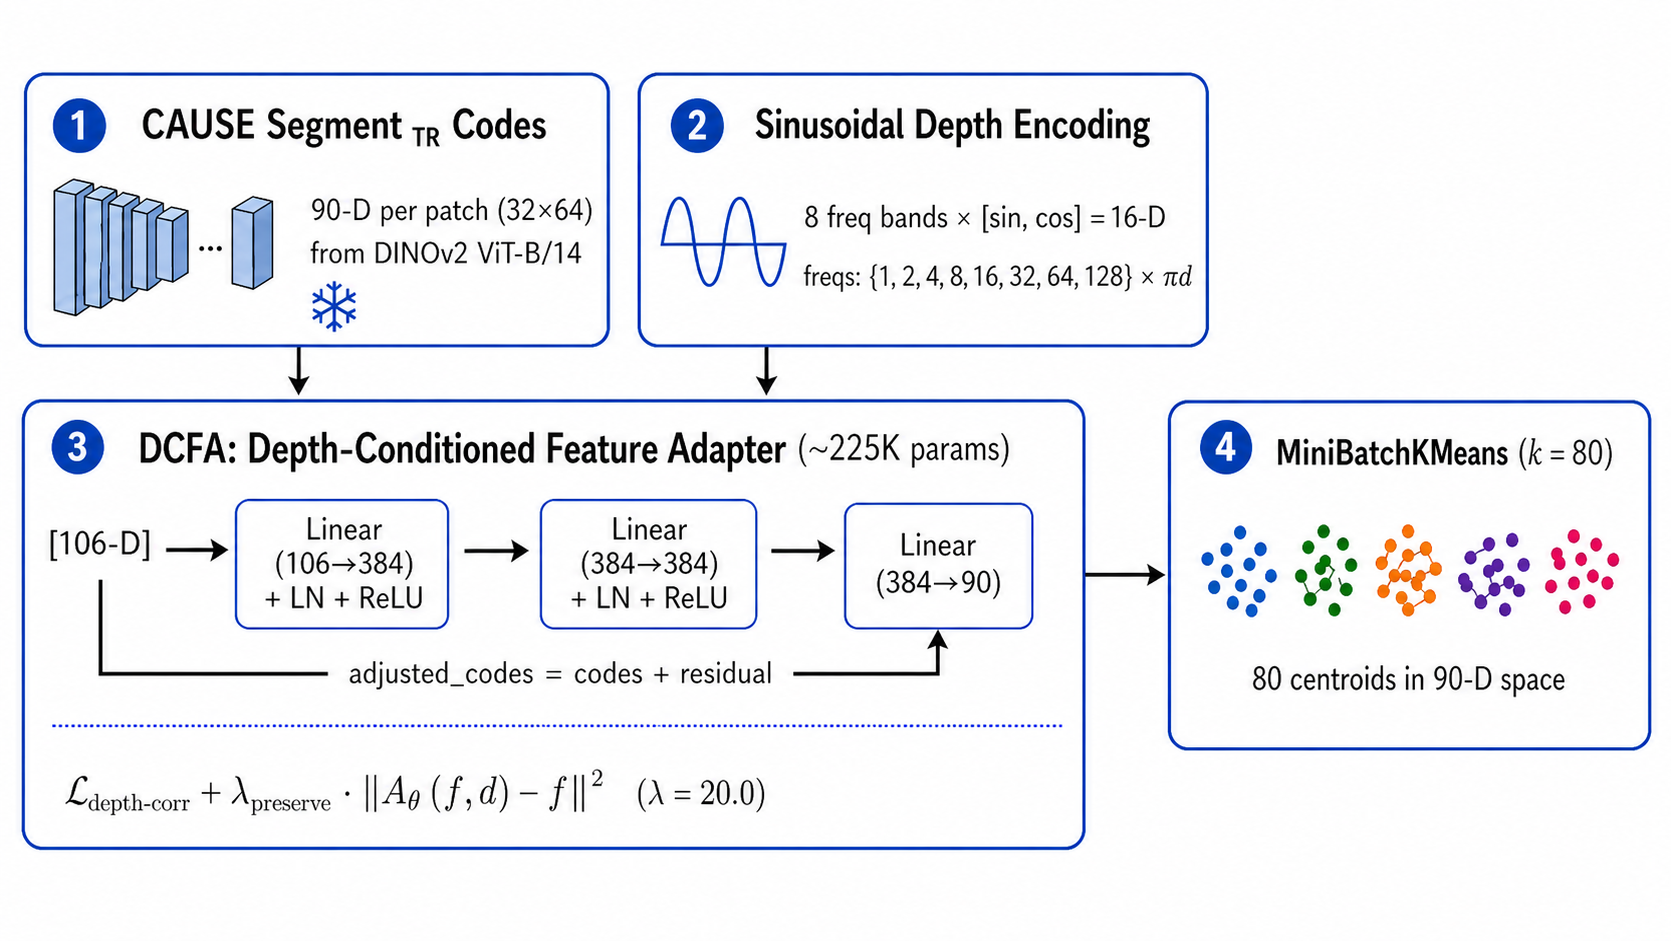
\includegraphics[width=\linewidth]{../figures/paper_ready/dcfa_adapter_training.png}
\caption{DCFA adapter training. A frozen CAUSE-TR code is adjusted by a depth-conditioned residual before $k$-means clustering, while a preservation term keeps the adapted code close to the original frozen semantic manifold.}
\label{fig:dcfa_adapter}
\end{figure}

The semantic regions inherited from the frozen CAUSE-TR code are appearance-driven, and the failure modes are: a single physical surface split across an illumination change, and two adjacent same-class objects merged into one region. Figure~\ref{fig:dcfa_adapter} summarizes the adapter path. We introduce a small residual adapter that consumes the depth value $d_u$ at pixel $u$ and adds a learned depth-driven shift to the frozen 90-dimensional code $z_u$, nudging cluster boundaries toward depth-consistent regions where appearance fails.

Conditioning on $d_u$ requires a representation rich enough for a small MLP to read both fine boundary differences and coarse depth ordering. Since $d_u \in [0, 1]$ is a scalar, we lift it through a 16-dimensional sinusoidal positional encoding with eight exponentially-spaced frequencies $\omega_k = 2^k \pi$ for $k = 0, \dots, 7$,
\begin{equation}
\begin{aligned}
e(d_u) = \big[ &\sin(\omega_0 d_u), \cos(\omega_0 d_u), \dots, \\
              &\sin(\omega_7 d_u), \cos(\omega_7 d_u) \big] \in \mathbb{R}^{16}.
\end{aligned}
\label{eq:sinusoid}
\end{equation}
The encoding $e(d_u)$ is concatenated with the frozen code $z_u$ into a 106-dimensional input, which a three-layer MLP $A: \mathbb{R}^{106} \to \mathbb{R}^{90}$ (two 384-wide hidden layers, each with layer normalization and ReLU, and a zero-initialized output projection) maps to a residual shift added to the frozen code,
\begin{equation}
\tilde z_u = z_u + A([z_u,\, e(d_u)]).
\label{eq:residual}
\end{equation}
The construction has approximately 225K (225,114) trainable parameters, small relative to the $\sim$86M parameters of the frozen ViT backbone. Because the output projection is zero-initialized, $\tilde z_u = z_u$ at the first optimizer step.

Training the adapter calls for a self-supervised signal that pulls the adapted codes of pixels at similar depth toward each other while keeping them on the original CAUSE-TR manifold. DepthG~\cite{sick2024depthg} established that depth-feature correlation can guide unsupervised semantic learning when depth governs the loss; we apply the same loss to the adapted code rather than to the backbone weights. For each minibatch image, we sample 1024 pixels and 1024 pixel pairs, using the DepthG depth-similarity kernel with bandwidth $\sigma_d = 0.5$. The adapter minimizes
\begin{equation}
\begin{aligned}
\mathcal{L}_\text{DCFA}
&= \mathcal{L}_\text{corr}(\tilde z, D)
 + \lambda_p \mathcal{L}_\text{preserve}(\tilde z, z), \\
\lambda_p &= 20 .
\end{aligned}
\label{eq:dcfa_loss}
\end{equation}
Here $\mathcal{L}_\text{corr}$ is the DepthG correlation loss on $(\tilde z,D)$, while $\mathcal{L}_\text{preserve}$ is the mean squared distance between $\tilde z$ and $z$.
\subsection{SIMCF: Semantic Instance Mutual Consistency Filtering}
\label{sec:method:simcf}

DCFA changes the feature space before clustering, but some errors remain after semantic and instance labels are formed. A depth fragment may cut through a single object, a proposal may contain pixels from multiple pseudo-classes, or a semantic assignment may sit at a depth far from the empirical range of its pseudo-class. SIMCF, short for Semantic Instance Mutual Consistency Filtering, is the final algorithm inside $G$: it takes the raw candidate pair $(S_x^0, I_x^0)$ and returns filtered pseudo-labels $(\hat S_x, \hat I_x)$ by enforcing consistency between semantic identity, instance geometry, feature similarity, and depth statistics.

Algorithm~\ref{alg:simcf} lists the procedure. The first check prevents mixed-class instance targets, the second repairs depth over-fragmentation using DINOv3 appearance similarity~\cite{simeoni2025dinov3}, and the third converts depth-implausible pixels into void labels rather than hard negatives. SIMCF has no learned parameters; DCFA remains the only learned component inside the Stage-1 generator, and the filtered labels are passed directly to panoptic bootstrapping.

\begin{figure*}[t]
\centering
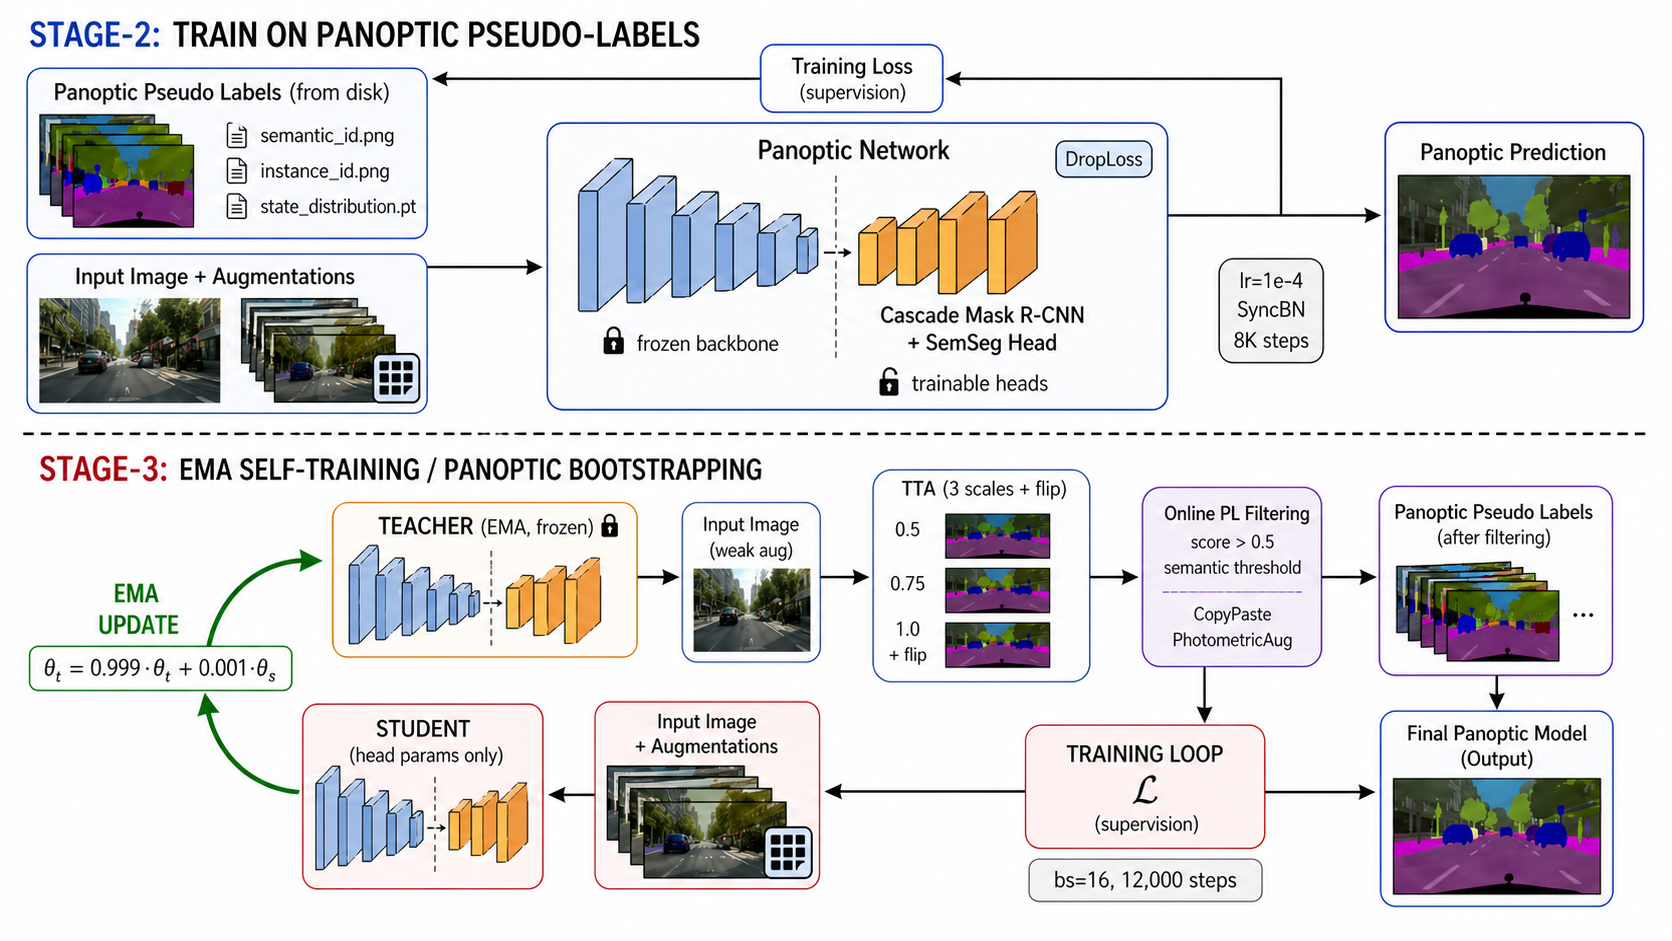
\includegraphics[width=0.90\textwidth]{../figures/paper_ready/panoptic_network_training.png}
\caption{Panoptic bootstrapping and panoptic network training. Filtered pseudo-labels supervise the initial panoptic network, and EMA self-training refines the labels and network across subsequent rounds, following the CUPS training recipe.}
\label{fig:panoptic_training}
\end{figure*}

\subsection{Panoptic Bootstrapping and Panoptic Network Training}
\label{sec:method:detector}

Filtering completes the Stage-1 generator $G$. The resulting pseudo-labels $(\hat S_x, \hat I_x)$ provide the supervision for panoptic bootstrapping, while the RGB image $x$ remains the network input. Figure~\ref{fig:panoptic_training} shows the training path adopted from CUPS. We adopt the panoptic bootstrapping and panoptic network training procedures from CUPS~\cite{hahn2025cups}, including its loss, copy-paste augmentation, bootstrapping schedule, and EMA self-training. Keeping these procedures fixed across configurations lets the experiments isolate the effect of the pseudo-label source.

The panoptic network takes $x$ as input and is trained on $(\hat S_x, \hat I_x)$. Its cascade, proposal, and panoptic heads use the CUPS-style losses; Section~\ref{sec:exp:setup} specifies the architecture.

\begin{cvpralgorithm}
\algorithmcaption{SIMCF$(S_x^0,I_x^0,D,\phi,v;\tau_\text{sim},\eta)$.}
\label{alg:simcf}
\begin{enumerate}
\setlength{\itemsep}{0pt}
\setlength{\topsep}{2pt}
\item $(\hat S_x,\hat I_x) \gets (S_x^0,I_x^0)$
\item \algkw{for each} instance region $R_k=\{p:\hat I_x(p)=k\}$ \algkw{do}
\item \algindent $c_k \gets \arg\max_c |\{p\in R_k:\phi(\hat S_x(p))=c\}|$
\item \algindent $s_k \gets \arg\max_s |\{p\in R_k:\hat S_x(p)=s,\ \phi(s)=c_k\}|$
\item \algindent \algkw{for each} $p\in R_k$ with $\phi(\hat S_x(p))\ne c_k$ \algkw{do}
\item \algindenttwo $\hat S_x(p)\gets s_k$
\item \algkw{for each} adjacent proposal pair $(a,b)$ in $\hat I_x$ \algkw{do}
\item \algindent compute mean features $\bar v_a,\bar v_b$ over $R_a,R_b$
\item \algindent \algkw{if} $c_a=c_b$ and $\cos(\bar v_a,\bar v_b)>\tau_\text{sim}$ \algkw{then}
\item \algindenttwo merge $R_a$ and $R_b$ in $\hat I_x$
\item \algkw{for each} pseudo-class $c$ \algkw{do}
\item \algindent $P_c\gets\{p:\phi(\hat S_x(p))=c\}$
\item \algindent $(\mu_c,\sigma_c)\gets(\operatorname{mean}D(P_c),\operatorname{std}D(P_c))$
\item \algkw{for each} pixel $p$ \algkw{do}
\item \algindent $c\gets\phi(\hat S_x(p))$
\item \algindent \algkw{if} $|D(p)-\mu_c|>\eta\sigma_c$ \algkw{then}
\item \algindenttwo $\hat S_x(p)\gets\mathrm{void}$; \quad $\hat I_x(p)\gets0$
\item \algkw{return} $(\hat S_x,\hat I_x)$
\end{enumerate}
\end{cvpralgorithm}

Two ingredients of the inherited recipe interact directly with the void labels produced by SIMCF. Following CUPS, DropLoss~\cite{wang2023cutler} masks losses on void or unreliable regions so that rejected pseudo-labels are not treated as hard negatives, making void a soft abstention rather than a class signal. Self-enhanced copy-paste augmentation operates at the input level: at each training iteration, instances from the pseudo-labels of one image are pasted into another image at random positions. This augmentation increases exposure to thing-class instances.

Once the cascade trainer reaches its bootstrapped checkpoint, three rounds of EMA self-training continue from it. In each round, an exponential-moving-average teacher is maintained over the student weights and used to relabel the unlabeled training set; the student is re-trained on the resulting refined pseudo-labels. The teacher provides a smoother, lower-variance label distribution than $G$ alone supplies, in particular for thing-class boundaries where Stage-1 labels are limited by monocular depth discontinuities. We use the final-round student checkpoint as the network $F$ in Eq.~\ref{eq:pipeline}.

At test time, $F$ takes a single RGB image $x$ and emits a dense semantic prediction over the pseudo-class vocabulary used for panoptic bootstrapping together with a set of instance proposals from the cascade heads. A panoptic merge step combines them into $(S_x, I_x)$ along the lines of~\cite{kirillov2019panoptic}: pixels assigned to thing-eligible pseudo-classes inherit the instance identifier of the highest-confidence instance proposal that covers them, pixels assigned to stuff pseudo-classes receive instance identifier 0, and overlapping instance proposals on the same pixel are resolved by confidence ranking. The pseudo-class outputs are mapped to benchmark classes only at evaluation time. Ground-truth annotations are used only for evaluation, including the Hungarian mapping from pseudo-classes to benchmark classes; they are never used to train $G$ or $F$.

Figure~\ref{fig:real_data_flow} traces the same data flow on real Cityscapes images, showing Stage-1 intermediate outputs together with the paired RGB/label transformations used by panoptic bootstrapping and panoptic network training.

\begin{figure*}[!t]
\centering
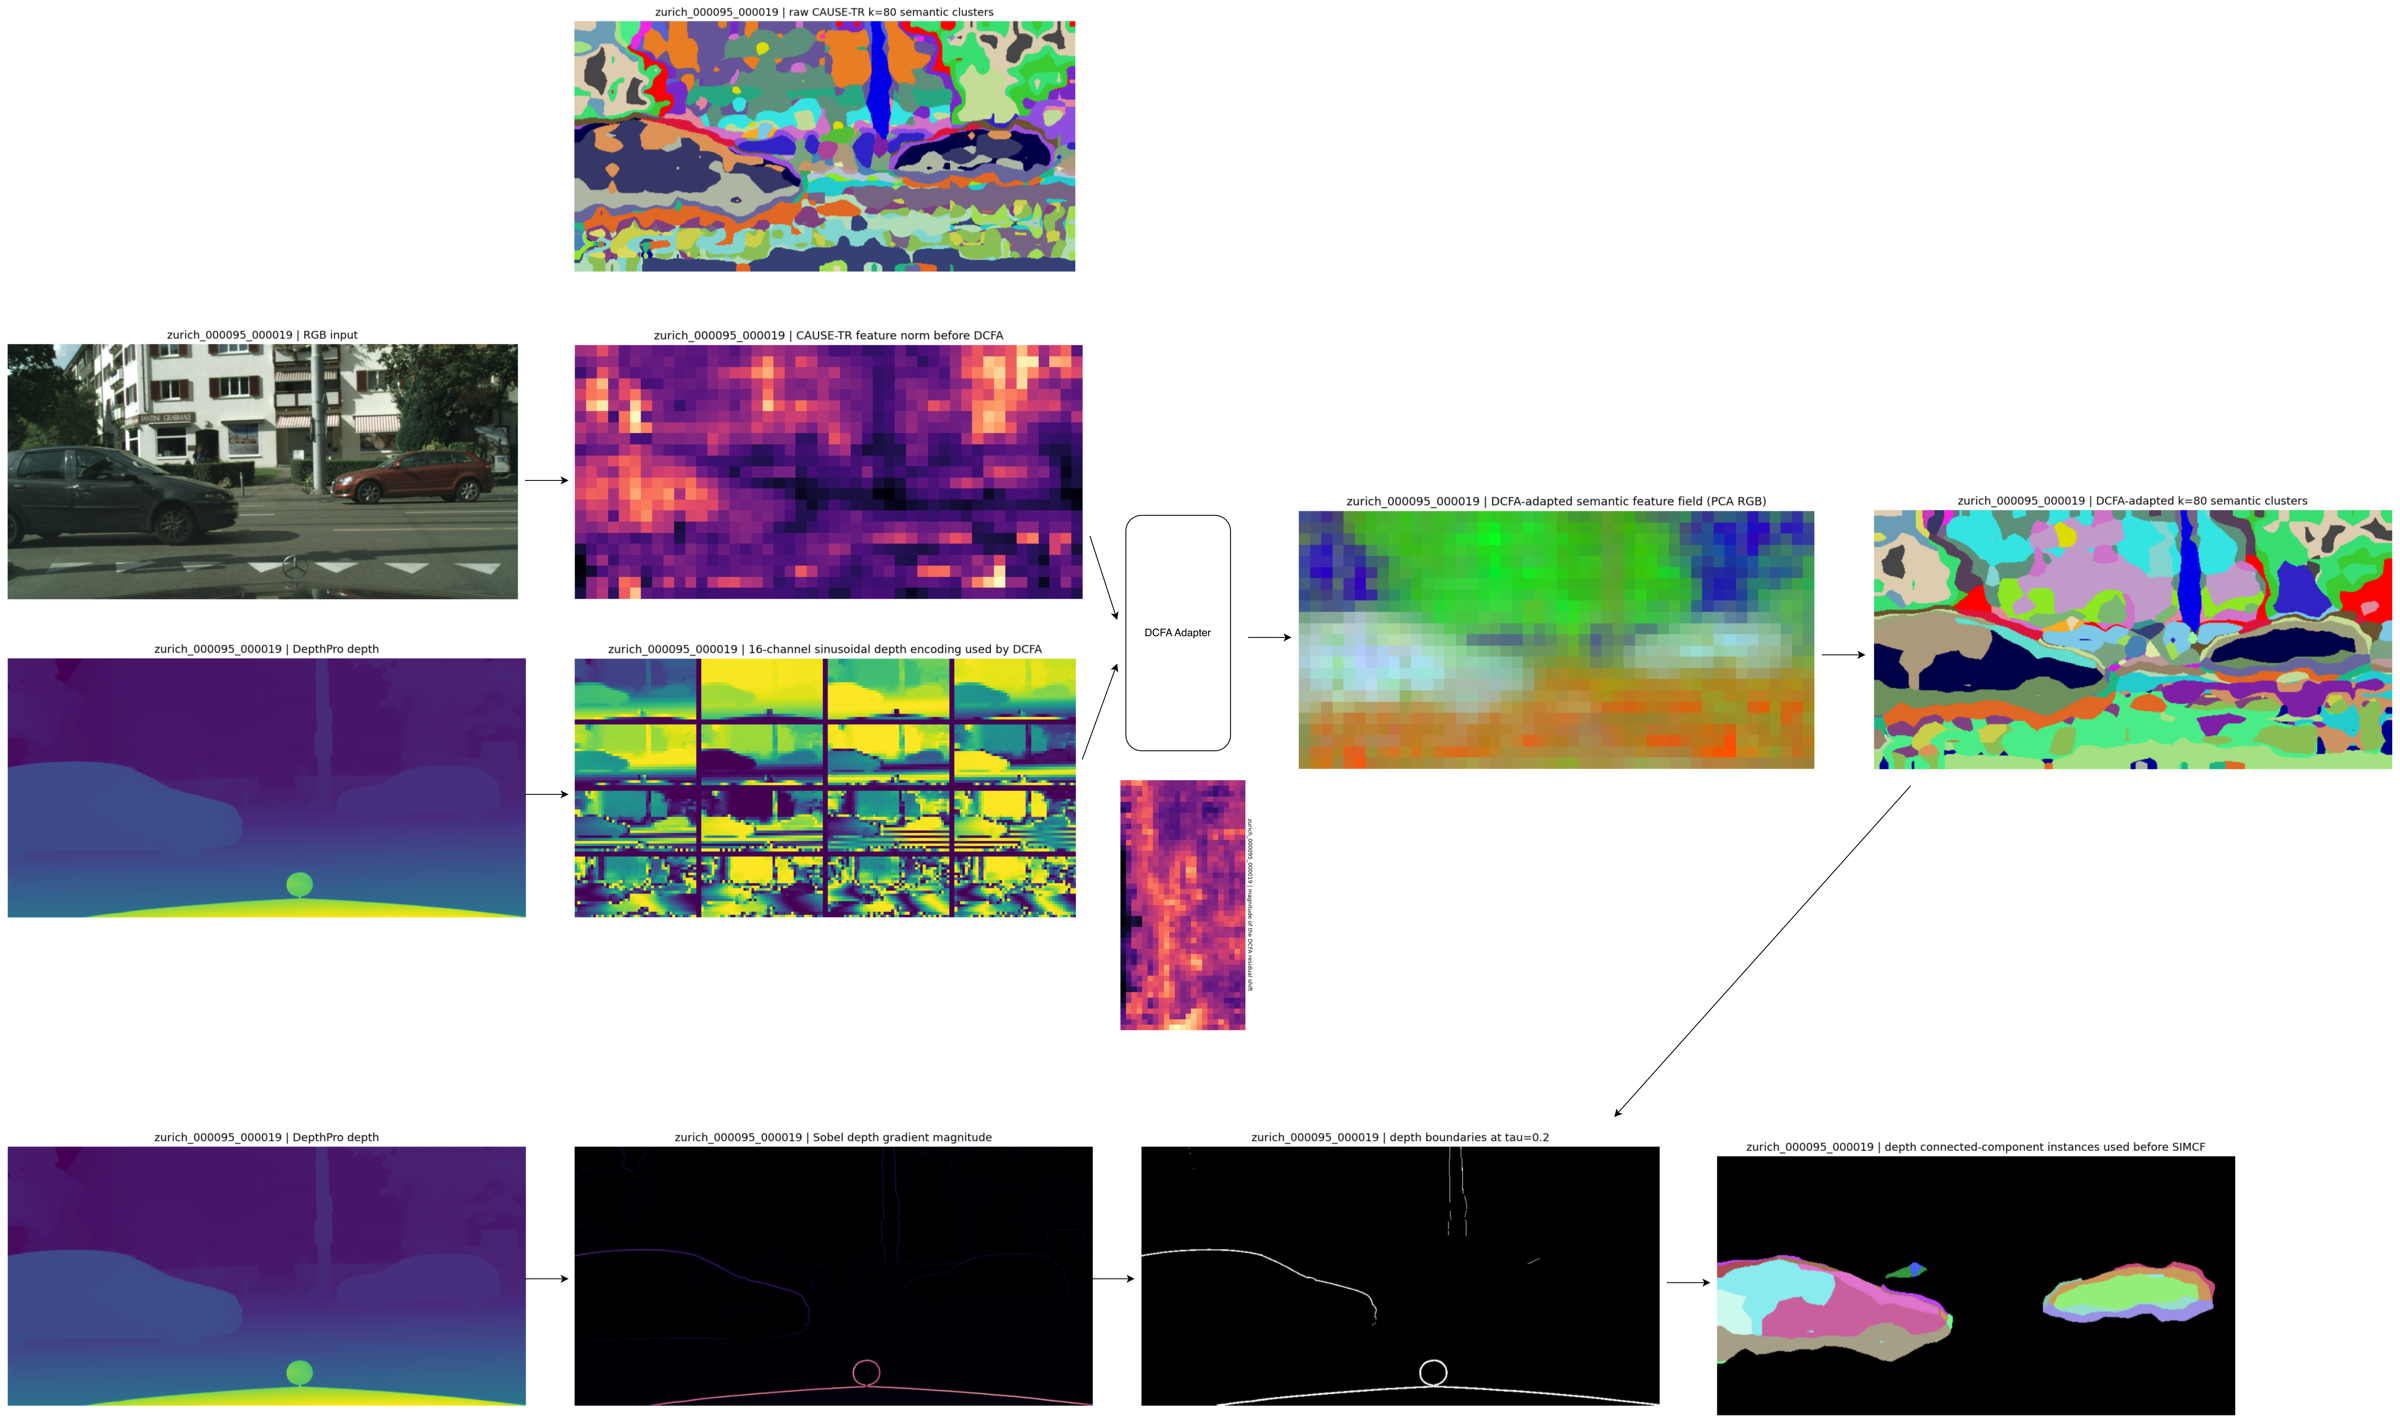
\includegraphics[width=0.62\textwidth]{../figures/paper_ready/pipeline_visualization_1_paper.png}\\[-2pt]
\footnotesize (a) Stage-1 pseudo-label trace, sample 1.\\[2pt]
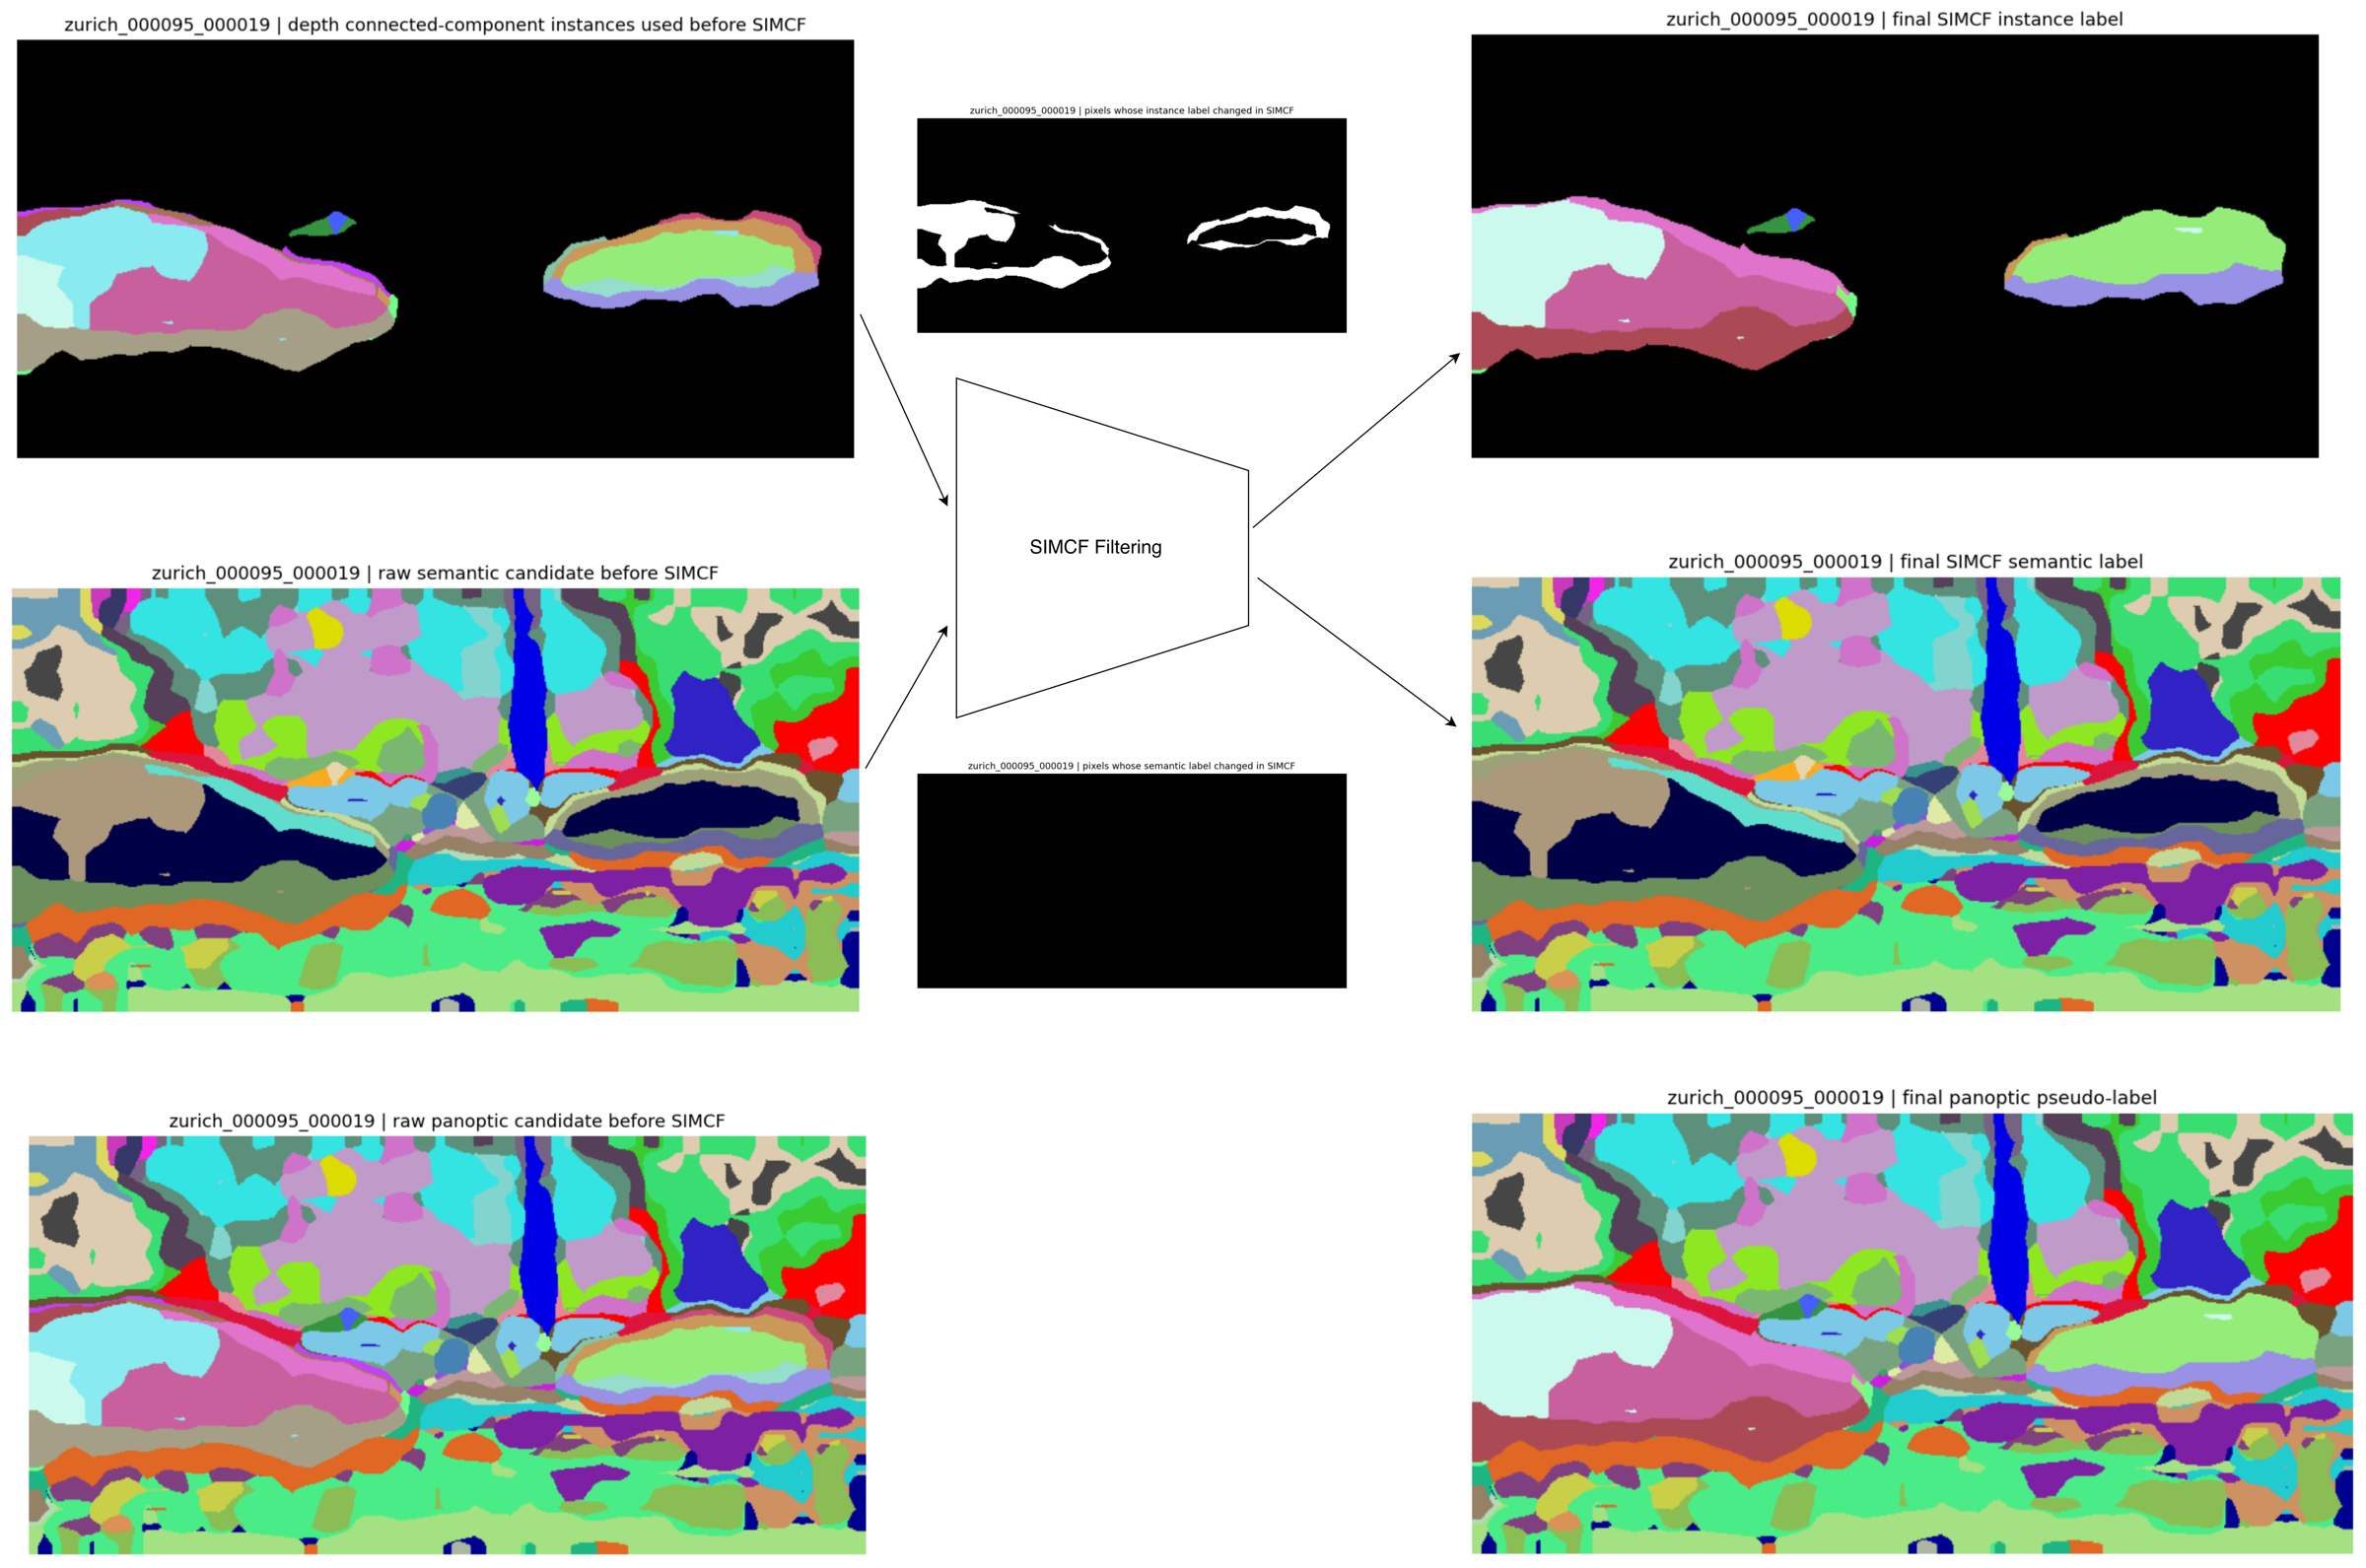
\includegraphics[width=0.62\textwidth]{../figures/paper_ready/pipeline_visualization_2_paper.png}\\[-2pt]
\footnotesize (b) Stage-1 pseudo-label trace, sample 2.\\[2pt]
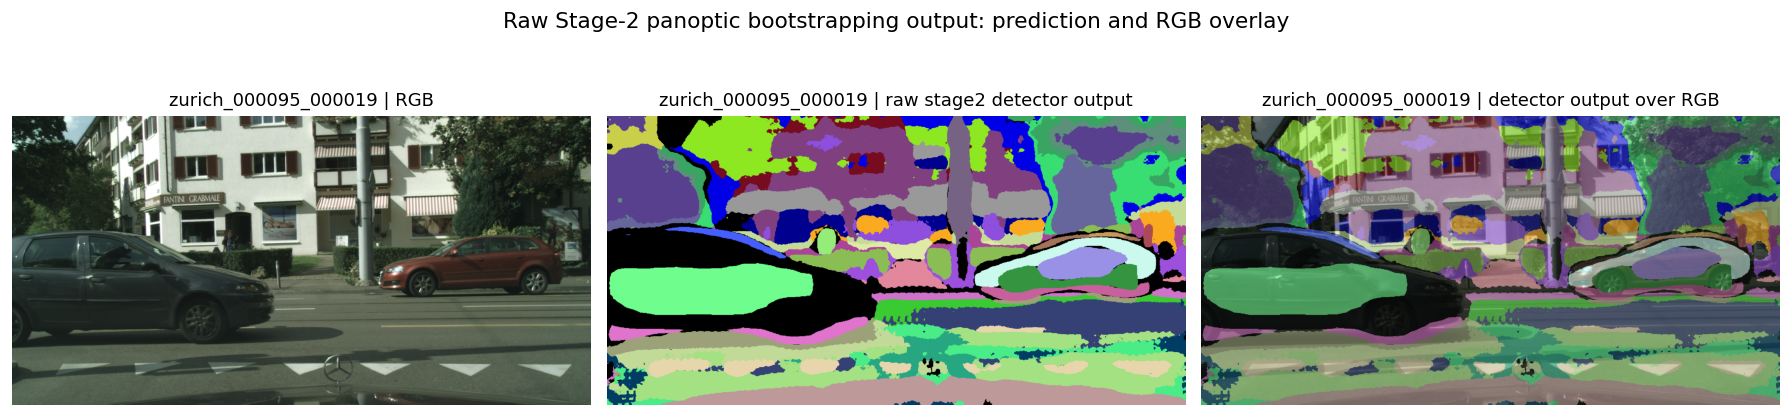
\includegraphics[width=0.62\textwidth]{../figures/paper_ready/stage_2_visualization_paper.png}\\[-2pt]
\footnotesize (c) Panoptic bootstrapping transformations.\\[2pt]
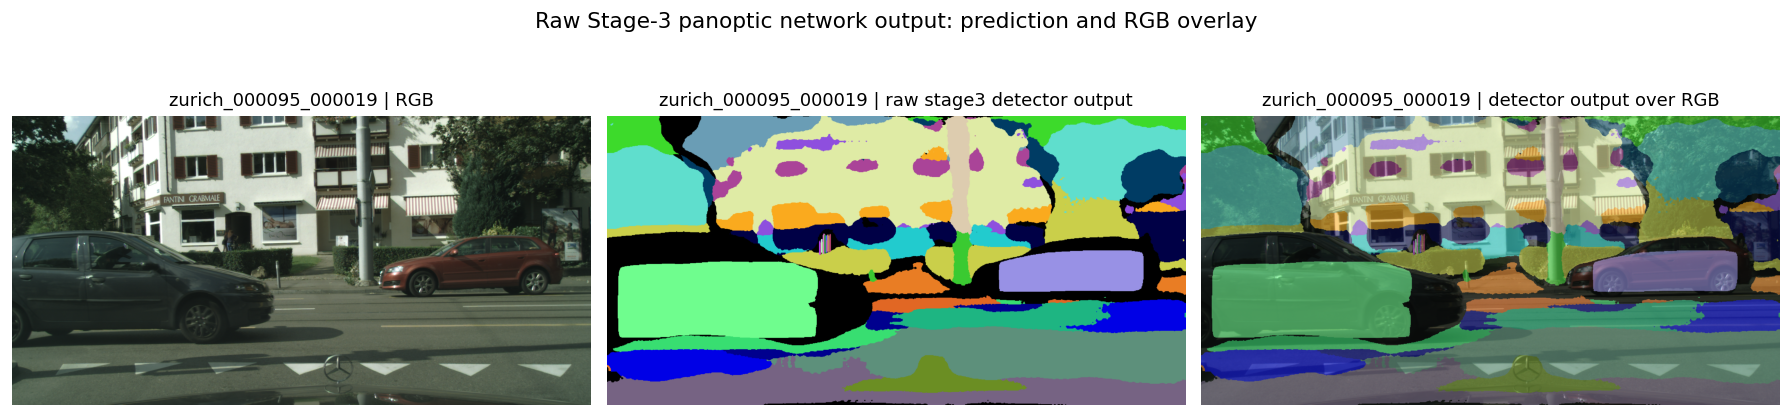
\includegraphics[width=0.62\textwidth]{../figures/paper_ready/stage_3_visualization_paper.png}\\[-2pt]
\footnotesize (d) Panoptic network-training transformations.
\caption{Real-image data flow. Panels (a) and (b) visualize how a monocular frame becomes semantic clusters, depth-derived instance candidates, SIMCF-filtered pseudo-labels, and an overlay. Panels (c) and (d) show the paired image/label transformations used when those pseudo-labels are consumed during panoptic bootstrapping and later EMA network training.}
\label{fig:real_data_flow}
\end{figure*}

%=========================================================================
\section{Experiments}
\label{sec:experiments}
%=========================================================================

We report experiments on Cityscapes and zero-shot transfer datasets, separating pseudo-label quality from trained-network performance. The evaluation asks whether monocular pseudo-labels can seed the adopted CUPS training procedure, how much DCFA and SIMCF contribute, and where the fixed Cityscapes-derived pseudo-class vocabulary fails.

\subsection{Experimental Setup}
\label{sec:exp:setup}

Pseudo-label generation and panoptic network training use only Cityscapes train~\cite{cordts2016cityscapes} (2,975 images, no annotations); evaluation reports Cityscapes val (500 images) under the 27-class CAUSE pseudo-vocabulary with a Hungarian map to Cityscapes' 19 evaluation classes~\cite{kirillov2019panoptic}, following CUPS. The Stage-1 generator $G$ uses a frozen DINOv2 ViT-B/14 backbone~\cite{oquab2024dinov2}, the frozen CAUSE-TR head~\cite{kim2024cause}, DCFA ($h = 384$, 16-D sinusoidal depth embedding, $\lambda_\text{preserve} = 20$, $\sim$225K trainable parameters trained for 10K iterations with AdamW at learning rate $10^{-3}$), $k$-means over-clustering at $k = 80$, the Section~\ref{sec:method:baseline} monocular instance branch with $\tau_d = 0.20$, $A_\text{min} = 1000$, and three iterations of dilation, and SIMCF ($\tau_\text{sim} = 0.85$, $\eta = 2.5$). DepthPro~\cite{bochkovskii2024depthpro} supplies the monocular depth map.

We follow CUPS for the training side. Panoptic bootstrapping denotes the initial training of a panoptic network on Stage-1 pseudo-labels with DropLoss~\cite{wang2023cutler} and self-enhanced copy-paste augmentation. Panoptic network training denotes the subsequent EMA self-training rounds, where teacher predictions relabel the training set and the student continues training on the refined labels. In both stages, the panoptic network is a Cascade Mask R-CNN~\cite{cai2018cascade} with three cascade stages on a frozen DINOv3 ViT-B/16 backbone~\cite{simeoni2025dinov3}; we use 8K bootstrapping steps followed by three 5K-step EMA rounds with EMA coefficient 0.999 and a three-scale teacher.


\subsection{Main Cityscapes Results}
\label{sec:exp:main}

Table~\ref{tab:main} records the main comparison on Cityscapes val. Rows 4--5 use the same panoptic bootstrapping and panoptic network training implementation defined above; only the Stage-1 pseudo-label source differs. DCFA+SIMCF add 3.07 PQ in this controlled comparison.

\begin{table*}[t]
\centering
\small
\setlength{\tabcolsep}{4pt}
\begin{tabular}{c l l l c c c c}
\toprule
\# & Method & Training & PL inputs & PQ & SQ & RQ & mIoU \\
\midrule
1 & U2Seg~\cite{niu2024u2seg} & published & RGB monocular & 18.4 & 55.8 & 22.7 & -- \\
2 & S2-UniSeg~\cite{xu2025s2uniseg} & published & RGB monocular & 25.4 & 66.7 & 35.0 & -- \\
3 & CUPS~\cite{hahn2025cups} & published & RGB + stereo + optical flow & 27.80 & 57.4 & 35.2 & 26.80 \\
4 & Monocular baseline (no DCFA, no SIMCF) & ours & RGB monocular & 32.76 & 62.57 & 40.75 & 45.14 \\
5 & Ours (DCFA + SIMCF) & ours & RGB monocular & 35.83 & 62.79 & 43.78 & 44.56 \\
\bottomrule
\end{tabular}
\caption{Cityscapes panoptic results. ``PL inputs'' are the inputs available at pseudo-label time. Published rows use metrics reported by the original papers; rows 4--5 isolate DCFA+SIMCF under the same panoptic bootstrapping and panoptic network training implementation.}
\label{tab:main}
\end{table*}

The final model is obtained after three EMA self-training rounds. Cityscapes validation improves from 31.87/60.84/39.94 (PQ/SQ/RQ) at step 800 to 33.77/61.75/42.04 at step 1000, 35.47/62.57/43.21 at step 2200, and 35.83/62.79/43.78 at step 3000. Most of the gain comes from recognition rather than mask quality: RQ rises by 3.84 points across this trajectory, while SQ rises by 1.95 points. The cross-row mIoU change (56.22 pseudo-label vs 44.56 trained-model) is not directly comparable because pseudo-label mIoU is computed against the 27-class CAUSE-TR vocabulary, while trained-model mIoU is computed under the 19-class Cityscapes evaluation.

Table~\ref{tab:perclass} reports the per-class validation metrics for the final step-3000 network. The aggregate gain is not uniform: large stuff regions and large vehicles combine high SQ with high RQ, while thin structures and rare classes are recognition-limited.

\begin{table*}[t]
\centering
\scriptsize
\setlength{\tabcolsep}{2pt}
\begin{tabular}{l c c c l c c c l c c c}
\toprule
Class & PQ & SQ & RQ & Class & PQ & SQ & RQ & Class & PQ & SQ & RQ \\
\midrule
road & 93.0 & 95.0 & 97.9 & tunnel & 0.0 & 0.0 & 0.0 & rider & 22.9 & 62.6 & 36.6 \\
sidewalk & 62.4 & 78.5 & 79.5 & pole & 2.0 & 72.3 & 2.8 & car & 70.7 & 88.7 & 79.7 \\
parking & 0.0 & 0.0 & 0.0 & polegroup & 0.0 & 0.0 & 0.0 & truck & 62.6 & 83.8 & 74.7 \\
rail track & 8.4 & 67.2 & 12.5 & traffic light & 6.2 & 60.3 & 10.3 & bus & 76.7 & 90.8 & 84.4 \\
building & 83.5 & 85.7 & 97.5 & traffic sign & 37.2 & 65.9 & 56.4 & caravan & 0.0 & 0.0 & 0.0 \\
wall & 32.3 & 67.7 & 47.8 & vegetation & 84.7 & 85.7 & 98.8 & trailer & 0.0 & 0.0 & 0.0 \\
fence & 20.3 & 63.0 & 32.1 & terrain & 35.7 & 73.4 & 48.6 & train & 77.2 & 88.7 & 87.0 \\
guard rail & 0.0 & 0.0 & 0.0 & sky & 86.1 & 89.9 & 95.7 & motorcycle & 0.1 & 100.0 & 0.1 \\
bridge & 17.2 & 64.5 & 26.7 & person & 13.4 & 71.4 & 18.7 & bicycle & 39.0 & 77.2 & 50.5 \\
\bottomrule
\end{tabular}
\caption{Per-class Cityscapes validation metrics for the final network. Values are percentages from the final step-3000 model used in Table~\ref{tab:main}.}
\label{tab:perclass}
\end{table*}


\subsection{Ablations}
\label{sec:exp:ablations}

\paragraph{Component contribution.}
Table~\ref{tab:components} reports DCFA $\times$ SIMCF at the fixed training-data instance configuration ($\tau_d = 0.20$). All four cells share the same depth instances; only the pre-clustering adapter and the post-instance filter are toggled. The logged single-component runs separate the behavior of the two corrections: DCFA raises SQ, while SIMCF raises RQ. The combined run has the best recorded pseudo-label PQ, consistent with the two stages targeting different failure modes.

\begin{table}[t]
\centering
\small
\setlength{\tabcolsep}{3pt}
\begin{tabular}{l c c c c c c}
\toprule
Variant & DCFA & SIMCF & PQ & SQ & RQ & mIoU \\
\midrule
Raw $K$=80 & -- & -- & 24.54 & 60.0 & 33.6 & 56.56 \\
DCFA only & \checkmark & -- & 25.22 & 61.0 & 34.0 & 56.16 \\
SIMCF only & -- & \checkmark & 25.27 & 57.5 & 34.4 & 56.57 \\
Both & \checkmark & \checkmark & 25.85 & 58.3 & 34.9 & 56.22 \\
\bottomrule
\end{tabular}
\caption{Pseudo-label component complementarity at fixed $\tau_d = 0.20$ DepthPro instances. ``Raw $K$=80'' is the no-DCFA, no-SIMCF baseline.}
\label{tab:components}
\end{table}

\paragraph{Depth model.}
Table~\ref{tab:depth} reports representative depth-source and threshold runs for which the evaluations provide aggregate SQ and RQ. The rows are not used as a single leaderboard because some runs use the raw $K$=80 semantic map and others use the DCFA semantic map; they are used to separate mask quality from recognition quality while choosing the training-data configuration.

\begin{table}[t]
\centering
\small
\setlength{\tabcolsep}{3pt}
\begin{tabular}{l l c c c c}
\toprule
Depth & Sem. & $\tau$ & PQ & SQ & RQ \\
\midrule
SPIdepth & raw $K$=80 & 0.20 & 26.74 & 71.88 & 31.41 \\
DA v3~\cite{lin2025da3} & raw $K$=80 & 0.03 & 27.37 & 73.44 & 35.66 \\
DA v3~\cite{lin2025da3} & DCFA & 0.20 & 26.44 & 61.37 & 35.83 \\
DepthPro~\cite{bochkovskii2024depthpro} & DCFA & 0.01 & 27.81 & 63.07 & 37.40 \\
DepthPro~\cite{bochkovskii2024depthpro} & DCFA & 0.20 & 26.13 & 60.63 & 35.80 \\
\bottomrule
\end{tabular}
\caption{Depth and threshold diagnostics with aggregate SQ/RQ.}
\label{tab:depth}
\end{table}

The table shows why PQ alone is not a sufficient diagnostic for the depth branch. The sharper $\tau = 0.01$ DepthPro setting has stronger standalone PQ/SQ/RQ, but it produces a fragmented training set with roughly 57 instances per image and more than half below 1000 pixels. The $\tau = 0.20$ setting has lower standalone PQ but produces larger training targets, roughly 22 instances per image, which is the configuration used for panoptic bootstrapping. DA v3 at the same training-data threshold reaches a similar RQ, indicating that the choice is governed by the training signal produced by the depth branch rather than by the stuff/thing aggregate split.


\subsection{Generalization and Failure Analysis}
\label{sec:exp:generalization}

\begin{table}[t]
\centering
\small
\setlength{\tabcolsep}{3pt}
\begin{tabular}{l r c c c c}
\toprule
Dataset & \# img & PQ & SQ & RQ & mIoU \\
\midrule
\multicolumn{6}{l}{\emph{Driving (comparable):}} \\
Cityscapes val & 500 & 35.83 & 62.79 & 43.78 & 44.56 \\
KITTI~\cite{geiger2012kitti} & 200 & 34.85 & 62.43 & 42.91 & 46.87 \\
Mapillary v2 & 2{,}000 & 39.19 & 74.59 & 47.74 & 58.87 \\
\midrule
\multicolumn{6}{l}{\emph{Sanity (NOT directly comparable):}} \\
MOTS~\cite{voigtlaender2019mots} & 2{,}862 & 61.10 & 88.71 & 65.80 & 92.10 \\
COCO-Stuff-27~\cite{caesar2018coco} & 1{,}000 & 7.83 & 38.55 & 10.06 & 14.22 \\
\bottomrule
\end{tabular}
\caption{Zero-shot cross-dataset transfer (no fine-tuning).}
\label{tab:transfer}
\end{table}

KITTI and Mapillary Vistas v2 show that the trained network transfers across the driving class space without retraining. KITTI stays close to Cityscapes across all three panoptic metrics, while Mapillary reaches higher SQ and RQ under its validation protocol. The MOTS row should not be read as a direct transfer score: MOTS evaluates a much narrower label space and therefore produces unusually high SQ and RQ. COCO-Stuff-27 shows the limit of the fixed pseudo-class vocabulary: a Cityscapes-derived $K = 80$ pseudo-label space cannot recover categories that were not represented during supervision, yielding only 10.06 RQ and 7.83 PQ.

\paragraph{Per-class failure analysis.}
The per-class table in Section~\ref{sec:exp:main} exposes the main failure modes. Large stuff (road, sky, vegetation, building) and large vehicles (car, bus, train) are strong, because frozen semantic codes give coherent regions and depth boundaries roughly coincide with object extent. Thin structures (pole, traffic light) and recognition-bottleneck classes (person, rider) are weak: monocular depth provides no separating discontinuity for co-planar pedestrians. Six classes are effectively dead --- parking, guard rail, tunnel, polegroup, caravan, and trailer --- because the $K = 80$ pseudo-label vocabulary after Hungarian alignment to the 27-class evaluation contains few or no positive examples for them.

Two qualitative metrics from the feature-guided merge step of SIMCF close the analysis. Average pseudo-instance count per image drops from 44 before the merge to 22 after, median instance size grows from 5{,}502 to 14{,}965 pixels, and stuff contamination falls from 50.7\% to 28.0\%. Many depth gradients are intra-object surface changes rather than object boundaries, and merging fragments whose semantic identity and dense appearance agree recovers the single-object structure that monocular depth had over-fragmented.


%=========================================================================
\section{Discussion}
\label{sec:discussion}
%=========================================================================

The results support three observations. First, cross-modal agreement improves monocular pseudo-labels at both feature and label levels. DCFA changes the semantic code before clustering, while SIMCF filters candidate labels after instance extraction. The component-complementarity table in Section~\ref{sec:exp:ablations} shows that the combined system improves pseudo-label PQ by +1.31 over the raw monocular baseline, more than either component alone. Under the fixed panoptic bootstrapping and network-training procedure, this pseudo-label improvement corresponds to a +3.07 PQ gain over the corresponding monocular baseline.

Second, monocular pseudo-labels are competitive in the driving-scene setting studied here. CUPS constructs pseudo-labels from stereo depth and unsupervised scene flow; our generator uses a single monocular depth map and frozen self-supervised features. The experiments show that this replacement is sufficient to train a strong panoptic network under the adopted CUPS procedure. A CUPS rerun under the same implementation in Section~\ref{sec:exp:setup} remains the decisive missing control, so the conclusion is intentionally narrow: for Cityscapes-style driving scenes, DepthPro depth and frozen DINO-family features can supply much of the structure that stereo and motion provided in CUPS.

Third, the remaining gap is concentrated in instance recognition for small and co-planar objects. Even with the full pipeline, person and rider remain at 13.37 and 22.94 per-class PQ, respectively. Monocular depth produces co-planar fragmentations on closely-spaced pedestrians, and CAUSE-TR's appearance-driven semantic code does not separate individual persons from a crowd. A finer instance signal, either monocular depth that resolves co-planar separations or a learned instance prior conditioned on individual-person geometry, would be required to close the rest.


%=========================================================================
\section{Limitations}
\label{sec:limitations}
%=========================================================================

\noindent Dead classes remain the main in-domain limitation: six classes in the 27-class pseudo-vocabulary receive too few reliable pseudo-labels, leaving them effectively absent after Hungarian alignment. This vocabulary limitation also explains the main out-of-domain failure. The Cityscapes-derived pseudo-label space transfers within driving scenes, but it fails on object-centric COCO-Stuff-27, where many categories are outside the supervision represented by the learned vocabulary.


%=========================================================================
\begin{thebibliography}{99}
%=========================================================================
\bibitem{cordts2016cityscapes} M.~Cordts, M.~Omran, S.~Ramos, et~al. The Cityscapes dataset for semantic urban scene understanding. \emph{CVPR}, 2016.
\bibitem{voigtlaender2019mots} P.~Voigtlaender, M.~Krause, A.~Osep, et~al. MOTS: Multi-object tracking and segmentation. \emph{CVPR}, 2019.
\bibitem{geiger2012kitti} A.~Geiger, P.~Lenz, R.~Urtasun. Are we ready for autonomous driving? The KITTI vision benchmark suite. \emph{CVPR}, 2012.
\bibitem{caesar2018coco} H.~Caesar, J.~Uijlings, V.~Ferrari. COCO-Stuff: Thing and stuff classes in context. \emph{CVPR}, 2018.
\bibitem{kirillov2019panoptic} A.~Kirillov, K.~He, R.~Girshick, et~al. Panoptic segmentation. \emph{CVPR}, 2019.
\bibitem{caron2021dino} M.~Caron, H.~Touvron, I.~Misra, et~al. Emerging properties in self-supervised vision transformers. \emph{ICCV}, 2021.
\bibitem{oquab2024dinov2} M.~Oquab, T.~Darcet, T.~Moutakanni, et~al. DINOv2: Learning robust visual features without supervision. \emph{TMLR}, 2024.
\bibitem{simeoni2025dinov3} O.~Sim\'eoni, et~al. DINOv3. \emph{arXiv}, 2025.
\bibitem{kim2024cause} J.~Kim, et~al. Causal unsupervised semantic segmentation. \emph{arXiv}, 2024.
\bibitem{bochkovskii2024depthpro} A.~Bochkovskii, et~al. Depth Pro: Sharp monocular metric depth in less than a second. \emph{arXiv}, 2024.
\bibitem{yang2024da2} L.~Yang, et~al. Depth Anything V2. \emph{NeurIPS}, 2024.
\bibitem{lin2025da3} D.~Lin, et~al. Depth Anything 3: Recovering the visual space from any views. \emph{arXiv}, 2025.
\bibitem{cai2018cascade} Z.~Cai, N.~Vasconcelos. Cascade R-CNN: Delving into high quality object detection. \emph{CVPR}, 2018.
\bibitem{wang2023cutler} X.~Wang, et~al. Cut and Learn for unsupervised object detection and instance segmentation. \emph{CVPR}, 2023.
\bibitem{wang2023tokencut} Y.~Wang, et~al. TokenCut: Self-supervised object discovery and instance segmentation. \emph{CVPR}, 2023.
\bibitem{hahn2025cups} A.~Hahn, et~al. Scene-centric unsupervised panoptic segmentation (CUPS). \emph{CVPR}, 2025.
\bibitem{niu2024u2seg} D.~Niu, et~al. Unsupervised universal image segmentation (U2Seg). \emph{CVPR}, 2024.
\bibitem{xu2025s2uniseg} Y.~Xu, et~al. S2-UniSeg. \emph{arXiv}, 2025.
\bibitem{sick2024depthg} N.~Sick, et~al. Unsupervised semantic segmentation through depth-guided feature correlation and sampling. \emph{CVPR}, 2024.
\bibitem{sick2025cuts3d} N.~Sick, et~al. CutS3D: Cutting semantics in 3D for 2D unsupervised instance segmentation. \emph{ICCV}, 2025.
\bibitem{hamilton2022stego} M.~Hamilton, et~al. STEGO: Unsupervised semantic segmentation by distilling feature correspondences. \emph{ICLR}, 2022.
\bibitem{ji2019iic} X.~Ji, et~al. Invariant information clustering for unsupervised image classification and segmentation. \emph{ICCV}, 2019.
\bibitem{cho2021picie} J.~Cho, et~al. PiCIE: Unsupervised semantic segmentation using invariance and equivariance in clustering. \emph{CVPR}, 2021.
\bibitem{seong2023hp} H.~Seong, et~al. Leveraging hidden positives for unsupervised semantic segmentation. \emph{CVPR}, 2023.
\bibitem{kim2024eagle} C.~Kim, et~al. EAGLE. \emph{arXiv}, 2024.
\bibitem{seong2024ppap} H.~Seong, et~al. PPAP. \emph{arXiv}, 2024.
\bibitem{couairon2024diffcut} P.~Couairon, et~al. DiffCut: Diffusion-feature partitioning. \emph{arXiv}, 2024.
\bibitem{bonnet2024hierarchy} L.~Bonnet, et~al. Recursive hierarchy clustering. \emph{arXiv}, 2024.
\bibitem{hoyer2021threeways} L.~Hoyer, et~al. Three ways to improve semantic segmentation with self-supervised depth estimation. \emph{CVPR}, 2021.
\bibitem{yin2025dformerv2} B.-W.~Yin, et~al. DFormerv2: Geometry Self-Attention for RGBD Semantic Segmentation. \emph{CVPR}, 2025.
\bibitem{simeoni2021lost} O.~Sim\'eoni, et~al. Localizing Objects with Self-Supervised Transformers and No Labels (LOST). \emph{BMVC}, 2021.
\bibitem{vangansbeke2022maskdistill} W.~Van~Gansbeke, et~al. MaskDistill. \emph{ECCV}, 2022.
\bibitem{wang2022freesolo} X.~Wang, et~al. FreeSOLO: Learning to segment objects without annotations. \emph{CVPR}, 2022.
\bibitem{arica2024cuvler} D.~Arica, et~al. CuVLER. \emph{CVPR}, 2024.
\bibitem{feng2025coler} Y.~Feng, et~al. COLER. \emph{arXiv}, 2025.
\bibitem{li2024promerge} X.~Li, et~al. ProMerge. \emph{arXiv}, 2024.
\bibitem{yang2025unmore} L.~Yang, et~al. unMORE. \emph{arXiv}, 2025.
\bibitem{wang2024unsam} X.~Wang, et~al. UnSAM. \emph{NeurIPS}, 2024.
\bibitem{yu2025unsamv2} J.~Yu, et~al. UnSAMv2. \emph{arXiv}, 2025.
\bibitem{seitzer2023dinosaur} M.~Seitzer, et~al. DINOSAUR: Bridging the gap to real-world object-centric learning. \emph{ICLR}, 2023.
\bibitem{gong2025mrdinosaur} S.~Gong, et~al. MR-DINOSAUR. \emph{arXiv}, 2025.
\bibitem{stone2021smurf} A.~Stone, et~al. SMURF: Self-teaching multi-frame unsupervised RAFT with full-image warping. \emph{CVPR}, 2021.
\bibitem{sommer2022sf2se3} L.~Sommer, et~al. SF2SE3: Clustering scene flow into SE(3)-motions via proposal and selection. \emph{GCPR}, 2022.
\end{thebibliography}

\end{document}
